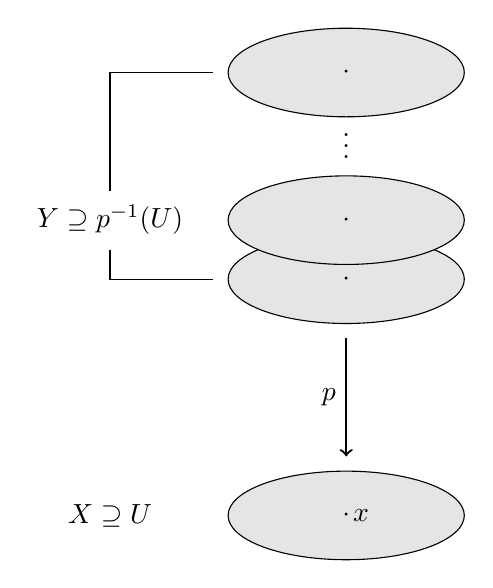
\begin{tikzpicture}[scale=0.75]
   \draw [black,fill=gray!20] (0,0)  ellipse (2cm and 0.75cm);
   \draw [black,fill=gray!20] (0,1) ellipse (2cm and 0.75cm);
   \draw [black,fill=gray!20] (0,3.5) ellipse (2cm and 0.75cm);
    \node at (0,2.4) {$\vdots$};
   \node at (0, 0) {$\boldsymbol{\cdot}$};
   \node at (0, 1) {$\boldsymbol{\cdot}$};
   \node at (0, 3.5) {$\boldsymbol{\cdot}$};
   \draw (-4,0.5) -- (-4,0) -- (-2.25,0);
   \draw (-4,1.5) -- (-4,3.5) -- (-2.25,3.5);
   \node at (-4, 1) {$Y \supseteq p^{-1}(U)$};

   \draw [thick,->] (0,-1) -- (0,-3) node[midway,left] {$p$};

   \draw [black,fill=gray!20] (0,-4)
      ellipse (2cm and 0.75cm);
   \node at (-4, -4) {$X \supseteq U$};
   \node at (0, -4) {$\boldsymbol{\cdot}$};
   \node at (0.25, -4) {$x$};

\end{tikzpicture}
